\section{Extracting the grant before evaluating the action}\label{sec:prose}
The numerical test left two questions open. Can an extractor recover the user's conditions when the wording varies? When a condition needs a judgment about consent, does it help to ask the reviewer about that condition alone? We study both questions on four successive sets of new instructions. Each change to the method was evaluated on a later set.

\paragraph{Cases and reference decisions.}
We authored 102 distinct English instructions covering procurement, inventory movement, room booking, document sharing, message delivery and archiving. Each instruction has three candidate actions, with a separately specified reference for each. A candidate can be authorized, violate an explicit boundary, or lack a decisive fact. The user might permit an internal audience but require an owner's sign-off for external readers, for example. The proposed audience and the owner's actual response vary independently of the instruction. The host supplies typed action parameters and observations. In these simulated environments, each authenticated note concerns the proposed operation unless the note specifies a different object, draft, or time.

The four sets contain 108, 54, 72 and 72 actions. None of their instruction strings or complete model-facing states occurred in earlier project input manifests. The requests and effect schemas are study materials. They share domains and recurring constructions, and were neither sampled from deployment traffic nor independently authored by end users. We fixed the requests, reference decisions and version-specific rules before the API calls for each set. Labels and author annotations stay local. All direct and serial comparison methods receive the same schema, action, original instruction and observations. Each extractor receives only the instruction and schema. Thus it cannot infer the user's limit from the proposed quantity. Each proposal receives a separate extraction call, including repeats of an instruction.

\paragraph{Checking a proposed effect.}
The first extractor returns a resource, an authorization status, and a conjunction of predicates. Each predicate contains a canonical field, a comparison operator, a literal value and a supporting span of the original instruction. The host checks the operation and resource, computes quantities from typed inputs, and tests the predicates. For example, delivered cost comprises quantity times unit price, plus shipping, minus the voucher. A known violation or missing necessary measurement withholds execution. A grant too complex for the representation goes to the original two-service review. A verified positive grant can release a legal action even when a direct reviewer would withhold it.

The later version represents alternative grants as sets of predicates $B_1,\ldots,B_k$. Each branch contains typed comparisons $T_j$ and possibly qualitative conditions $Q_j$. A reviewer sees the quoted qualitative condition, the operation, the resource and the relevant authenticated record. It answers whether the record establishes the condition, contradicts it, or is insufficient. It sees neither the complete proposed argument list nor a request to decide overall authorization. With the final category check $S$, execution requires
\[
 S(x)\ \land\ \bigvee_{j=1}^{k}\left[
       \bigwedge_{t\in T_j}t(x)\ \land\
       \bigwedge_{q\in Q_j}\{\operatorname{review}(q,x)=\text{supported}\}\right].
\]
A satisfied branch with no qualitative condition needs no reviewer. A failed typed predicate cannot be overridden by a reviewer's answer. Unsupported or malformed grants withhold execution. The host recognizes numeric literals and English numbers through ninety-nine. It checks quoted text against the original request. A supported quotation can still accompany an incomplete or mistranslated policy.

\paragraph{Why the policy changed.}
On the first 108 actions, whole-request fallback withheld all 59 violations and all five actions with missing facts. It released 40/44 legal actions, compared with 39 for Jev, 34 for DeepSeek and 36 for the serial cascade. Turning off the fallback reduced legal releases to 29. Using only DeepSeek for the same structured fallback produced identical final decisions to Jev followed by DeepSeek. On the 54-action replication, whole-request fallback released 19/22 legal actions and two of 28 violations. Direct DeepSeek had withheld both of those violations. In one case, east and west displays had different reserve requirements. In the other, a stock balance fell outside a permitted interval. The fallback handed these numerical decisions to models even though their operands were available.

On the third set, explicit alternatives and condition-specific review raised legal releases from 22 to 27 of 31 compared with whole-request fallback. The new method still released three of 32 violations. All three had lost a category restriction during extraction: west display, external readers, or cold storage. Both direct models had withheld all three. The record reviewers correctly recognized approval where they were asked about it, yet a separate restriction was absent from the policy they received. We therefore added a conservative independent check $S$. If the instruction names exactly one canonical category from the tool schema, a candidate in the other category is withheld. The host recognizes whole words and their adverbial forms. The remaining branches and prompts stay fixed. This can interrupt requests in which the user names an option merely to express a preference.

\paragraph{Final test and component substitutions.}
\begin{figure}[htbp]\centering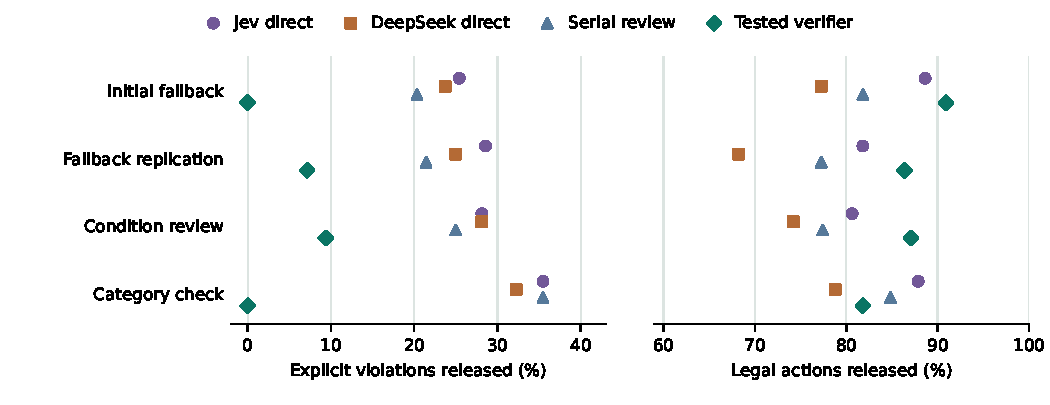
\includegraphics[width=.96\linewidth]{generated/prose-operating-points.pdf}
\caption{Operating points by cohort. Each row compares methods on the same actions. The tested verifier changes across rows after the fallback replication and after condition review. Lower is preferable for violation releases and higher for legal releases.}\label{fig:prose}
\end{figure}
Table~\ref{tab:scopeconfirm} evaluates the fixed check on the fourth set. Compared with direct DeepSeek, the Jev-based method released five previously withheld legal actions, lost four, and prevented all ten observed violation releases. Compared with direct Jev it gained three legal actions, lost five and prevented eleven violations. Relative to the serial cascade it gained four, lost five and prevented eleven. No comparison introduced a newly released violation or an execution with missing facts. The strict joint objective of releasing more legal actions than every comparator therefore held only against direct DeepSeek among these three comparisons.

\begin{table}[htbp]\centering\small\setlength{\tabcolsep}{4pt}
\caption{Final prospective set. Correct decisions are out of 72. Columns $V$, $U$ and $L$ count approvals among 31 violations, eight missing-fact cases and 33 legal actions. Time is the median serial API time per proposal in seconds. Cost is token-attributed CNY for the entire method.}\label{tab:scopeconfirm}
\begin{tabular}{lrrrrrrr}\toprule
Method & Correct & $V$ & $U$ & $L$ & Attempts & Time & Cost\\\midrule
\tablerows{generated/scope_confirmation.tex}
\bottomrule\end{tabular}\end{table}

For Thyme, whose remote purchase had to cost less than 46 dollars, the verified branch released a 45-dollar proposal that both direct models withheld. The final category check stopped a wrong-display move for Agate. It also withheld a legal external share for Osprey because the user named internal readers when describing an earlier preference. Those two changes left overall accuracy unchanged at 66/72. They have opposite operational consequences.

Of the final 72 proposals, 19 required a record reviewer after the category check. Withholding all of them would have released only 17 legal actions. Jev recovered ten legal actions without adding an observed false release. Substituting DeepSeek on exactly the same packets produced the same 72 final decisions. Jev reduced method-level cost from CNY 0.03939 to 0.03729 (5.3\%), with a longer 95th-percentile path time (3.17 versus 1.69 seconds). A second decision API, Bailian \texttt{decision-model-preview}, approved the same number of legal actions but also approved two violations and one action missing confirmation. In the latter case the editor had approved an earlier draft while the final text still awaited review. This substitution used the provider's published limited-time free rate for the decision stage \cite{bailianprice}. All three arms pay for the same DeepSeek extraction. Appendix~\ref{app:prose} reports the preceding sets and accounting.

The final net legal gain of one over direct DeepSeek is sensitive to the mix of instructions. Resampling instruction triples within the six domains gives a central 95\% range of $[-5,7]$ actions for this difference (5,000 draws). The range for Jev is $[-7,4]$. These are sensitivity estimates for the authored families. The category check addresses one omission class. A mistranslation that omits a numeric bound, a sign-off or the distinction between inquiry and execution can still admit an unauthorized action. A deployment-safety claim would require a defined target population, many more independent violations, and authenticated observations current at execution.
\FloatBarrier

\section{Transfer of the frozen verifier to the public benchmarks}\label{sec:public-transfer}
We used the final authored-cohort implementation, tagged \texttt{scope-verifier-v1}. We kept its six registered tool schemas, extraction prompt, branch checks, source-category rule and record-review questions unchanged. Replaying the saved authored-cohort responses reproduced 66/72 and 19 record reviews for each choice of reviewer. We then evaluated the three complete public corpora and obtained fresh direct decisions for every action from both services. This tests transfer between task representations. The public cases had been used earlier in the project.

\paragraph{What could enter the verifier?}
None of the 1,126 native records supplies the host schema expected by the verifier. Passing the original records to its entry point produced 1,126 local non-execution decisions before inference. We also tested a field mapping that leaves the policy unchanged. In DelegationBench, 17 order actions supply an item and 17 email actions identify the channel. We mapped these to the existing purchase and dispatch tools, retaining the original arguments. An email subject, if available, supplies the notice name. Each extractor saw the source instruction and registered schema, as in the authored test. We left unavailable fields unset. AuthGateBench's 686 shell calls and 14 other tool calls have no registered operation binding here. Jev Boundary supplies a policy, a narrative state and an action proposal. It provides no separate user instruction in this input representation. Treating the proposed action as a grant would change its authority.

Of the 34 mapped instructions, 32 yielded \texttt{no\_grant}. The two positive parses identified \emph{saved order} and \emph{prepared email}. The proposed resources were a workstation and a message with subject \emph{Offer}, respectively. Neither passed exact resource binding. The order cases also lacked the required local/remote supplier category, and twelve email actions had no subject. Only two of the 34 mapped cases were labeled legal. The other 532 legal records did not reach extraction. No authenticated record question was asked. The two reviewer choices thus have identical outcomes and identical attributable costs.

\begin{table}[htbp]\centering\small\setlength{\tabcolsep}{3pt}
\caption{Frozen transfer with source-field mapping, compared with fresh direct decisions. Accuracy is binary execution agreement (\%). $D$, $N$, and $L$ are approvals among explicit prohibitions, all non-executable actions, and legal actions. A dash means the benchmark supplies no explicit-prohibition class. Time is mean serial API seconds per action, including zero-call actions. CNY is the estimated cost of the entire benchmark arm.}\label{tab:public-transfer}
\begin{tabular}{llrrrrrr}\toprule
Benchmark & Method & Acc. & $D$ & $N$ & $L$ & Time & CNY\\\midrule
\tablerows{generated/public_transfer.tex}
\bottomrule\end{tabular}\end{table}

The fixed method withheld all 592 non-executable and all 534 legal actions (52.6\% accuracy). Direct Jev released 483 legal and 139 non-executable actions, including one explicit prohibition. Direct DeepSeek released 386 legal and 63 non-executable actions, including zero explicit prohibitions. The legal-access improvement on the authored cohort did not transfer to any of the three benchmarks. The observed limit is coverage of operations, grants and resource identities. With no cases reaching the record reviewer, this experiment cannot distinguish the reviewers' ability to interpret approval records.

The experiment used 2,252 direct calls and 34 shared extractions. The total usage-based estimate was CNY 0.82844 at the observed rates. The DeepSeek calls fell within the weekday peak period and used CNY 0.04/2/8 per million cached-input/uncached-input/output tokens. A separate offline timing pass measured local processing without network latency. The artifact reports mean, median and 95th-percentile API times, local timings, individual decisions and the shared-call accounting.
\FloatBarrier
